\documentclass[]{article}
\usepackage{proceed2e}

\usepackage{times}
\usepackage{cite} 

\usepackage{tikz} 
\usepackage{varwidth}
\usepackage{paralist}
\usepackage{comment}


\usepackage{graphicx}
\usepackage{epstopdf}
\usepackage{caption}
\usepackage{subcaption}
% \usepackage{fixltx2e}
% \usepackage{dblfloatfix} 

\newcommand{\sectionspace}{\vspace{-0.3cm}}
\newcommand{\plotspace}{\vspace{-0.25cm}}

\usepackage{color}
\newcommand{\todo}[1]{{\small\color{red}[#1]}}

%CHEAT CODES
\renewcommand{\baselinestretch}{.98}
% \renewcommand{\textfloatsep}{0.5ex}

\title{Calibration-Free BCI based Control using Error Related Potentials}

\author{
\bf{Jonathan Grizou} \\ Inria Bordeaux Sud-Ouest, France \\ jonathan.grizou@inria.fr
\And \bf{I\~naki Iturrate} \\ CNBI, EPFL, Switzerland \\ inaki.iturrate@epfl.ch\\
\AND \bf{Pierre-Yves Oudeyer} \\ Inria Bordeaux Sud-Ouest, France \\ pierre-yves.oudeyer@inria.fr
\And \bf{Manuel Lopes} \\ Inria Bordeaux Sud-Ouest, France \\ manuel.lopes@inria.fr
\And \bf{Luis Montesano} \\ I3A, Univ. of Zaragoza, Spain \\ montesano@unizar.es
}

\begin{document}
\maketitle

% \section{How will the projects be scored?}

The jury scores the submitted projects on the basis of a list of criteria. Your project should get high scores in one or more of the criteria to get a high ranking. Thus you may consider the following points when writing your submission:

\begin{itemize}
    \item does the project include a novel application of the BCI?
    \item is there any new methodological approach used compared to earlier projects?
    \item is there any new benefit for potential users of a BCI?
    is there any improvement in terms of speed of the system (e.g. bit/min)?
    \item is there any improvement in terms of accuracy of the system?
    \item does the project include any results obtained from real patients or other potential users?
    \item is the used approach working online/in real-time?
    \item is there any improvement in terms of usability?
    \item does the project include any novel hardware or software developments?
\end{itemize}

% \begin{abstract}
% Recent works have explored the use of brain signals to directly control virtual and robotic agents in sequential tasks. So far in such brain-computer interfaces (BCI), an explicit calibration phase was required to build a decoder that translates raw electroencephalography (EEG) signals from the brain of each user into meaningful instructions. We propose a new methodological approach that removes the calibration phase. The proposed method assumes a distribution of possible tasks, and infers the interpretation of EEG signals and the task by selecting the hypothesis which best explains the history of interaction. We report experiments where four users use BCI to control an agent on a virtual world to reach a target without any previous calibration process.
% \end{abstract}

\section{Introduction}
\sectionspace

EEG-based brain-computer interfaces have been used successfully to control different devices, such as robotic arms and simulated agents, using self-generated (e.g. motor imagery) and event-related potentials signals (see \cite{millan2010combining} for a review). Error-related potentials (ErrPs) are one kind of event-related potential appearing when the user's expectation diverges from the actual outcome. Recently, they have been used as feedback instructions for devices to solve a user's intended task \cite{chavarriaga2010learning,iturrate2010single}.

% \cite{Falkenstein00}

As in most BCI applications, ErrP-based BCI requires a calibration phase to learn a decoder  that translates raw EEG signals from the brain of each user into meaningful instructions. This calibration is required due to specific characteristics of the EEG signals: non-stationary nature, large intra- and inter-subject variability, and variations induced by the task. The presence of an explicit calibration phase, whose length and frequency is hard to tune and is often tedious and impractical for users, hinders the deployments of BCI applications out of the lab. Thus, calibration free methods are an important step to apply this technology in real applications \cite{millan2010combining}.

We propose a new methodological approach that removes the need for a calibration phase, this allows to simultaneously and seamlessly learn an EEG decoder of error-related potentials while controlling a device to achieve a sequential task. Contrary to other approaches \cite{kindermans2012bayesian}, our method learns the specific sequence of actions that fulfills the user's desired task. The proposed method assumes a distribution of possible tasks, and infers the interpretation of EEG signals and the task by selecting the hypothesis which best explains the history of interaction. This inference can be continuously run and updated as new data comes in, which removes the need for an explicit calibration. We report online experiments where four users use BCI to control in real time an agent on a virtual world to reach a desired target by following a trajectory without any previous calibration process. 

% Our method does not only learn to classify the EEG signals but also use them to learn a sequential task by following the preferences of the users, which makes it different from the work of Kindermans et al. \cite{kindermans2012p300}.

\sectionspace
\section{Principle}
\sectionspace

BCI control based on feedback signals differs from classical brain-computer interfaces in the sense that the user does not actively deliver commands to the device, but only delivers feedback about actions performed by the device \cite{chavarriaga2010learning,iturrate2010single}. Essentially, this BCI control follows an iterative sequential process where the device performs an action which is in turn assessed by the user. This assessment will elicit ErrPs into the user's brain that can be recorded using EEG and will be different for ``correct'' and ``incorrect'' assessments. 

This process can be exemplified for a reaching task, where the user wants to reach a target position unknown by the system. The device performs several discrete actions (e.g. moving left or right), and learns from the feedback given by the user. To solve this problem, the usual methods require a calibration phase to train a usable decoder of brain signals. Once the brain signals can be translated into binary feedback, the device can infer which sequence of actions can lead to the user's desired position. 

We explain how we can achieve similar performances without knowing the brain signal decoder beforehand. The intuition for our method  is that the classification of the brain signals is easier when they are interpreted according to the task desired by the user \cite{grizou2014calibration}. The method assumes a distribution of possible tasks and relies on finding which pair of decoder-task has the highest expected classification rate on the brain signals.

\label{sec:Algorithm}
\begin{figure}[!ht]
\centering
    \begin{tabular}{c|c|c}
        \begin{subfigure}[t]{0.29\columnwidth}
            \begin{flushleft}
            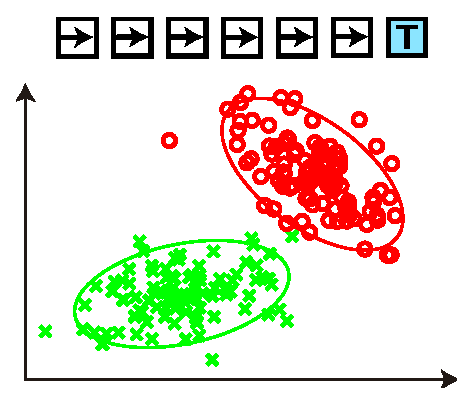
\includegraphics[width=\columnwidth]{img/GM1}
            \caption{}
            \label{fig:GM1}
            \end{flushleft}
        \end{subfigure}
        &
        \begin{subfigure}[t]{0.29\columnwidth}
            \begin{center}
            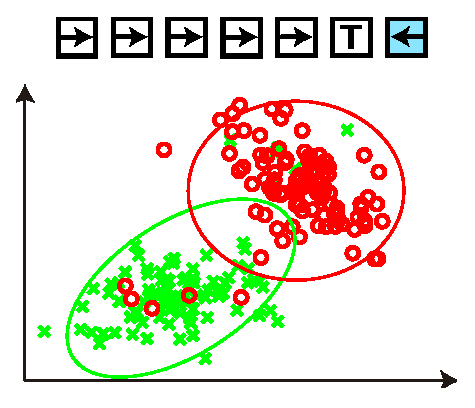
\includegraphics[width=\columnwidth]{img/GM2}
            \caption{}
            \label{fig:GM2}
            \end{center}
        \end{subfigure}
        &
        \begin{subfigure}[t]{0.29\columnwidth}
            \begin{flushright}
            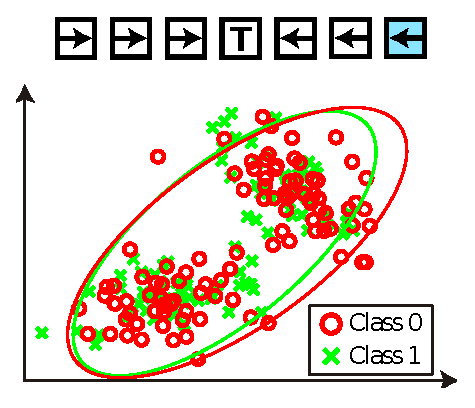
\includegraphics[width=\columnwidth]{img/GM3}
            \caption{}
            \label{fig:GM3}
            \end{flushright}
        \end{subfigure}
    \end{tabular}
\caption[]{Interpretation hypothesis for a 1D grid world. \plotspace}
% Representation of the interpretation hypothesis for a 1D grid world. Three task hypotheses are displayed from left to right [(a),~(b),~(c)]. On top is a 1D world with the hypothetic target state marked with a T letter. The user intended target is shown as the shaded blue state at the right extremity of the 1D world. The correct hypothesis is the one on the Left [(a)] where the T state is the same as the shaded blue state. Below the 1D grid world, the signals received from the user are represented in a 2D feature space. They represent the user assessment signals of the past history of device's actions (e.g.\ moving randomly left and right). Our algorithm assigns virtual labels (green for ``correct'' and red for ``incorrect'') to those signals with respect to their respective hypothetic target. We can compute the corresponding 2D Gaussian distributions for each class (shown as colored ellipses) and each hypothesis. While for the correct hypothesis [(a)] the Gaussian distributions shows a large separability, the overlap increases as the hypothetic target (T) moves away from the real (blue shaded) one [(b), (c)].}
\label{fig:GM}
\end{figure}

The main idea is depicted in Figure~\ref{fig:GM} for a toy 1D example. The user wants the device to reach the right-most state (shaded in blue). For each device's action, the user provides a feedback signal which encodes whether the action executed is ``correct'' or ``incorrect'' according to the intended target (represented in a 2D feature space). Such signals are generated from an underlying model which maps a binary label to a continuous signal. However, neither the user's desired target nor the labels associated to the user's feedback signals are known.

% (e.g. reaching one of a finite number of states)

Considering that we can define a finite set of target state hypothesis (marked with a T letter), we can infer the labels that should be provided by the user with respect to each hypothesis. Given a particular interaction history, it is possible to compute a different signal decoder for each task hypothesis. The key point is that only the correct hypothesis will assign the correct labels to all feedback signals (Figure~\ref{fig:GM1}), while the other hypotheses will gradually mix both classes as the hypothetic target gradually differs more from the correct one (Figure~\ref{fig:GM2}~and~\ref{fig:GM3}). 

Therefore, the hypothesis which provides the decoder with best accuracy and compactness can be selected as the most probable one. This property can be exploited by measuring the overlap between the distributions of each class \cite{grizou2014calibration}, by using for example the Bhattacharyya coefficient. The task intended by the user being the one whose associated signal models overlap the less.

\sectionspace
\section{Method}
\sectionspace

\paragraph{Control task} We consider a 5x5 grid world, where an agent can perform five different discrete actions: move up, down, left, right, or a target-reached action. The user wants to command the system to move to a particular location (i.e. to reach one of the 25 discrete states) following a trajectory and for this he/she can only use the brain feedback. 

% The user goal is to teach the agent the path to reach one of the 25 discrete states which represent the set of possible tasks (i.e. one hypothesis per possible target state).

\paragraph{EEG-based feedback signals} During operation, the role of the users was to mentally assess the agent's actions as correct or incorrect with respect to a selected target, obtaining this way error-related potentials. EEG signals were recorded with a gTec system (2 gUSBamp amplifiers) with 32 electrodes distributed according to the 10/10 international system, with the ground on FPz and the reference on the left earlobe. The EEG signals were digitized with a sampling frequency of $256$ Hz, common-average-reference filtered and band-pass filtered at $[0.5, 10]$ Hz.

\sectionspace
\section{Results}
\sectionspace

\paragraph{Comparison with calibration method}

Figure~\ref{fig:sequence} shows one particular run of 500 steps comparing our self-calibration method with a calibration procedure of 400 steps in simulation and using a pre-recorded dataset of ErrP signals. As our algorithm is operational from the first step, it can identify the correct task when sufficient evidence has been collected. On the other hand, a calibration approach collects signal-label pairs for a fixed number of steps and use the resulting classifier. During the calibration phase no tasks can be learned, substantially delaying the user's online operation. Importantly after the 500 steps the decoders of each methods are of similar qualities.

\begin{figure}[!ht]
\centering
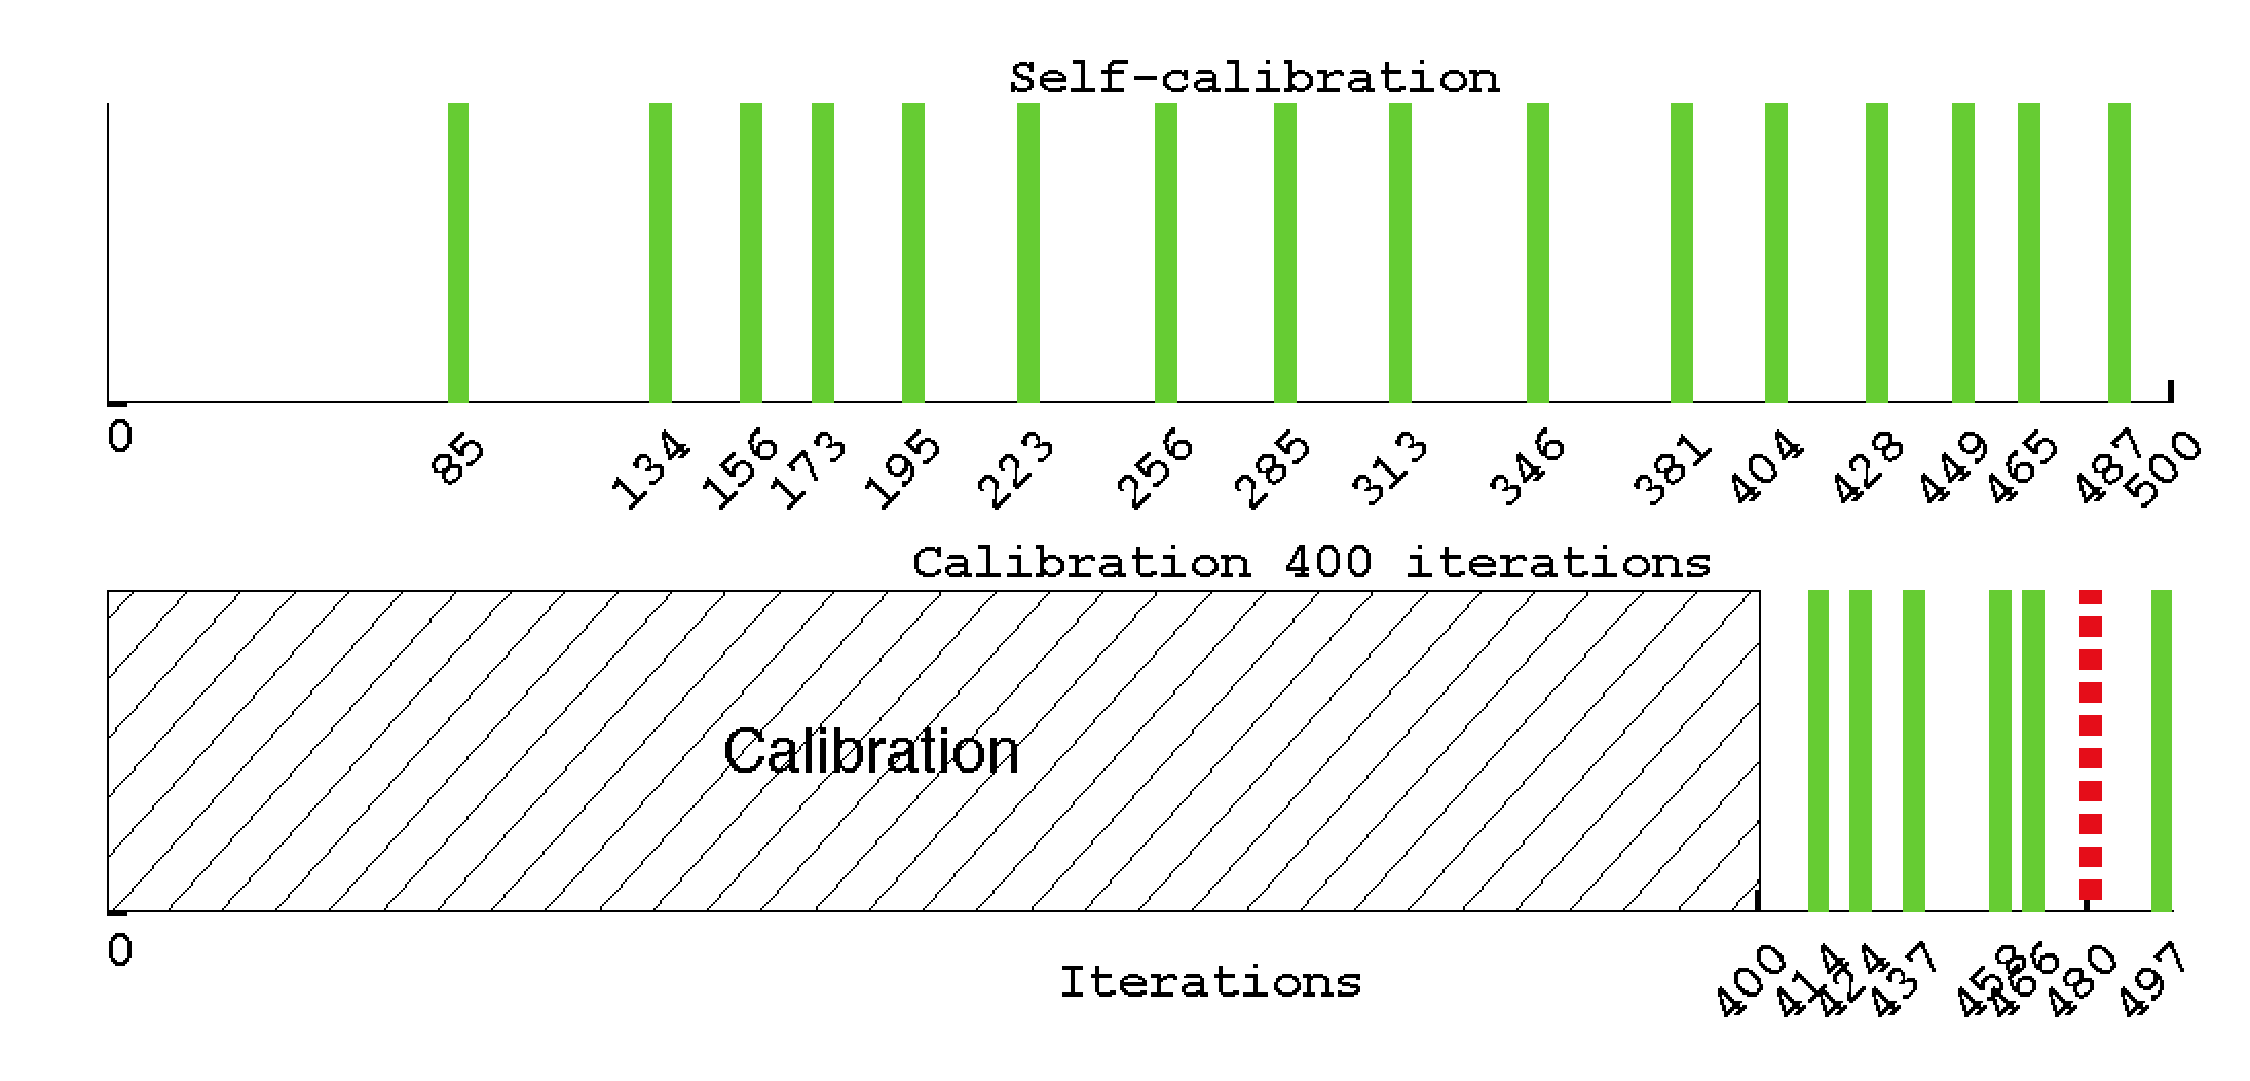
\includegraphics[width=\columnwidth]{img/plot_the_aaai_sequence.eps}
\caption{Time-line of one simulated experiment using an EEG dataset, self-calibration (top) versus calibration (bottom). Green (filled) and red (dashed) bars represents respectively correct and incorrect task achievement. \plotspace}
\label{fig:sequence}
\end{figure}

\paragraph{Calibration-Free Online BCI Control}

The experiments were conducted with four subjects (aged between 25 and 28). Each subject was asked to mentally assess the agent's actions with respect to a given target. Each subject performed 5 runs, for each run a new target, unknown to our system, was selected by the user. The system was not calibrated to decode the user EEG signals beforehand. There was an agent's action every three seconds. Each run lasted 200 actions, and the time between runs was around one minute.

Table~\ref{ch6tab:steps} shows for each subject and run the number of iterations needed to reach the confidence threshold for the subject selected target. The algorithm was able to identify the correct target for all runs of all the subjects.  On average, the number of iterations needed to identify the target was of 85 $\pm$ 32. We note that our system identified each task in less iterations than a normal calibration phase requires (between 300 and 600 examples depending on the user performance \cite{chavarriaga2010learning,iturrate2010single}).

\begin{table}[!ht]
\centering
\begin{footnotesize}
\begin{tabular}{r|rrrrr|r}
    %\toprule
    & \textbf{Run1} & \textbf{Run2} & \textbf{Run3} & \textbf{Run4} & \textbf{Run5} & \textbf{mean$\pm$std} \\\hline
    %\midrule
    \textbf{S1} & 95 & 62 & 56 & 60 & 64 & 67 $\pm$ 16 \\
    \textbf{S2} & 89 & 77 & 98 & 60 & 62  & 77 $\pm$ 17 \\
    \textbf{S3} & 68 & 80 & 118 & 76 & 157 & 100 $\pm$ 37 \\
    \textbf{S4} & 98 & 142 & 57 & 142 & 47 & 97 $\pm$ 45 \\
    %\bottomrule
\end{tabular}
\end{footnotesize}
  \caption{Number of iterations needed to identify the target for each subject and run. \plotspace}
  \label{ch6tab:steps}
\end{table}

% \sectionspace
% \section{Conclusion}
% \sectionspace

% This work opens new perspectives regarding the global challenge of interacting with machines. It has application to many interaction problems which requires a machine to learn how to interpret unknown communicative signals. A promising avenue, outside the BCI field, lies in human robot interaction scenarios where robots must learn from, and interact with, many different users who have their own limitations and preferences.

% \cite{grizou2013robot}

\sectionspace

\begin{footnotesize}
\bibliographystyle{ieeetr}
\bibliography{bciaward}
\end{footnotesize}

\end{document}


% Our main contribution is a calibration-free BCI method that infers simultaneously and seamlessly an EEG decoder of error-related potentials while controlling a device to achieve a sequential task. The core idea of the method is to assume a distribution of possible tasks, and infer the interpretation of EEG signals and the task by selecting the hypothesis which best explains the history of interaction. This inference can be continuously run and updated as new data comes in, which removes the need for an explicit calibration.

% We also present an evaluation of this method with online experiments where four users control an agent in a virtual world. The results show that the proposed method allows to learn a good signal decoder and solve the task efficiently without any explicit calibration. Offline experiments show that our unsupervised trained decoder achieves similar performances than calibration based systems and illustrate the benefits of our planning strategy for speeding up learning.

% We introduced a novel method for calibration-free BCI based control of sequential tasks with feedback signals. The method provides an unsupervised way to train a decoder with almost the same performance as state-of-the-art supervised classifiers, while keeping the system operational and solving the task requested by the user since the beginning. The intuition for our method is that the classification of the brain signals is easier when they are interpreted according to the task desired by the user. The method assumes a distribution of possible tasks and relies on finding which pair of decoder-task has the highest expected classification rate on the brain signals.

% The algorithm was tested with real online experiments, showing that the users were able to guide an agent to a desired position by mentally assessing the agent's actions and without any explicit calibration phase. Offline experiments show that we can identify an average of 20 tasks in 400 iterations without any calibration, while in previous works the calibration phase used between 300 and 600 examples. To improve the efficiency of the algorithm, we introduced a new planning method that uses the uncertainty in the decoder-task estimation. Finally, we analyzed the performance of the system in the presence of abrupt changes in the EEG signals. Our proposed method was able to adapt and reuse its learned models to the new signals. Furthermore, in those cases when the transfer is not possible, our method can still be used to recalibrate the system from scratch while solving the task.

% A current limitation of the work is the need for a finite set of task hypotheses. This limitation could be solved by the use of a combination of particle filter and regularization on the task space. Additionally, our method can not dissociate fully symmetric hypotheses, e.g.\ right and left most state of our 1D grid world (Fig. \ref{fig:GM}), as the interpretation of feedback signals will also be symmetric and therefore as likely. This latter problem can be solved by redefining the set of hypotheses or the action set, for instance by adding a ``stop'' action valid only at the target state.

% In this paper we have shown that, given a limited number of possible tasks, it is possible to solve sequential tasks using human feedback without defining a map between feedback signals and their meaning beforehand. 


% @inproceedings{grizou2013robot,
%     title = {{Robot learning simultaneously a task and how to interpret human instructions}},
%     author = {Grizou, Jonathan and Lopes, Manuel and Oudeyer, Pierre-Yves},
%     booktitle = {{Joint IEEE International Conference on Development and Learning and on Epigenetic Robotics (ICDL-EpiRob)}},
%     year = {2013}
% }

% @inproceedings{iturrate2010single,
%   title={{Single trial recognition of error-related potentials during observation of robot operation}},
%   author={Iturrate, Inaki and Montesano, Luis and Minguez, Javier},
%   booktitle={Engineering in Medicine and Biology Society (EMBC), 2010 Annual International Conference of the IEEE},
%   pages={4181--4184},
%   year={2010},
%   organization={IEEE}
% }


% @article{chavarriaga2010learning,
%   title={{Learning from EEG error-related potentials in noninvasive brain-computer interfaces}},
%   author={Chavarriaga, Ricardo and J.d.R. Mill\'an},
%   journal={Neural Systems and Rehabilitation Engineering, IEEE Transactions on},
%   volume={18},
%   number={4},
%   pages={381--388},
%   year={2010},
%   publisher={IEEE}
% }

% @article{millan2010combining,
%   title={{Combining brain-computer interfaces and assistive technologies: state-of-the-art and challenges}},
%   author={Mill{\'a}n, J.d.R. and Rupp, R{\"u}diger and M{\"u}ller-Putz, Gernot R and Murray-Smith, Roderick and Giugliemma, Claudio and Tangermann, Michael and Vidaurre, Carmen and Cincotti, Febo and K{\"u}bler, Andrea and Leeb, Robert and others},
%   journal={Frontiers in neuroscience},
%   volume={4},
%   year={2010},
%   publisher={Frontiers Research Foundation}
% }

% @ARTICLE{Falkenstein00,
%   author = {M. Falkenstein AND J. Hoormann AND S. Christ AND J. Hohnsbein},
%   title = {{ERP components on reaction errors and their functional significance: A tutorial}},
%   journal = {Biological Psychology},
%   year = {2000},
%   volume = {51},
%   pages = {87-107}
% }

% @inproceedings{grizou2014calibration,
%     title = {{Calibration-Free BCI Based Control}},
%     author = {Grizou, Jonathan and Iturrate, I{\~n}aki and Montesano, Luis and Oudeyer, Pierre-Yves and Lopes, Manuel},
%     booktitle = {{AAAI Conference on Artificial Intelligence}},
%     year = {2014}
% }

% @inproceedings{kindermans2012p300,
%   title={{A P300 BCI for the Masses: Prior Information Enables Instant Unsupervised Spelling.}},
%   author={Kindermans, Pieter-Jan and Verschore, Hannes and Verstraeten, David and Schrauwen, Benjamin},
%   booktitle={NIPS},
%   pages={719--727},
%   year={2012}
% }


